\subsection{Reconstruction des points}
\begin{frame}{Triangulation : retrouver les coordonnées 3D}
\begin{minipage}[t]{0.48\textwidth}
  \vspace*{\fill}
  \begin{itemize}
    \item<1-> On connaît les matrices de projection \( P_1 \) et \( P_2 \)
    \item<2-> Deux points image correspondants :
    \[
      x_1 = (u_1, v_1),\quad x_2 = (u_2, v_2)
    \]
    \item<3-> Inconnue : \( X = (x_C, y_C, z_C) \) point 3D
    \item<4-> On pose :
    \[
      \lambda_1 x_1 = P_1 X,\quad \lambda_2 x_2 = P_2 X
    \]
    \item<5-> Cela donne un système de 6 équations linéaires homogènes
  \end{itemize}
  \vspace*{\fill}
\end{minipage}
\hfill
\begin{minipage}[t]{0.50\textwidth}
  \only<4->{
  \[
  \begin{cases}
  \lambda_1 u_1 = p_{11}^{1} x_C + \dots + p_{14}^{1} \\
  \lambda_1 v_1 = p_{21}^{1} x_C + \dots + p_{24}^{1} \\
  \lambda_1 = p_{31}^{1} x_C + \dots + p_{34}^{1} \\
  \lambda_2 u_2 = p_{11}^{2} x_C + \dots + p_{14}^{2} \\
  \lambda_2 v_2 = p_{21}^{2} x_C + \dots + p_{24}^{2} \\
  \lambda_2 = p_{31}^{2} x_C + \dots + p_{34}^{2}
  \end{cases}
  \]
  }
\end{minipage}
\end{frame}

\begin{frame}{Triangulation : formulation du système}
\vspace*{-0.5em}
\begin{itemize}
  \item<1-> Une fois \( P_1 \) et \( P_2 \) déterminées,
  \item<2-> On cherche les coordonnées \( X = (x_C, y_C, z_C, 1)^T \)
  \item<3-> Pour chaque paire \( (x_1, x_2) \) de projections
  \item<4-> On élimine \( \lambda_1, \lambda_2 \) et on écrit un système homogène
  \item<5-> Système sous la forme \( A X = 0 \)
\end{itemize}

\vspace{1em}

\pause
\pause
\pause
\pause
\begin{center}
\scriptsize
\[
A =
\left(
\begin{array}{cccc}
p_{31}^{1} u_1 - p_{11}^{1} & p_{32}^{1} u_1 - p_{12}^{1} & p_{33}^{1} u_1 - p_{13}^{1} & p_{34}^{1} u_1 - p_{14}^{1} \\
p_{31}^{1} v_1 - p_{21}^{1} & p_{32}^{1} v_1 - p_{22}^{1} & p_{33}^{1} v_1 - p_{23}^{1} & p_{34}^{1} v_1 - p_{24}^{1} \\
p_{31}^{2} u_2 - p_{11}^{2} & p_{32}^{2} u_2 - p_{12}^{2} & p_{33}^{2} u_2 - p_{13}^{2} & p_{34}^{2} u_2 - p_{14}^{2} \\
p_{31}^{2} v_2 - p_{21}^{2} & p_{32}^{2} v_2 - p_{22}^{2} & p_{33}^{2} v_2 - p_{23}^{2} & p_{34}^{2} v_2 - p_{24}^{2}
\end{array}
\right)
\]
\end{center}
\end{frame}

\begin{frame}{Triangulation : résolution}
\vspace*{-0.5em}
\begin{itemize}
  \item<1-> On résout le système \( A X = 0 \)
  \item<2-> Solution obtenue par la SVD de \( A \)
  \item<3-> Le vecteur \( X \) est donné par :
  \[
    X = \text{dernier vecteur colonne de } V \text{ dans } A = U \Sigma V^T
  \]
  \item<4-> On homogénéise : \( X \leftarrow \frac{1}{X_4} X \)
  \item<5-> Répété pour chaque paire de points \( (x_1, x_2) \)
  \item<6-> On obtient la reconstruction 3D des points
\end{itemize}
\end{frame}

\begin{frame}{Reconstruction 3D multi-vues}
  \begin{minipage}{0.6\linewidth}
    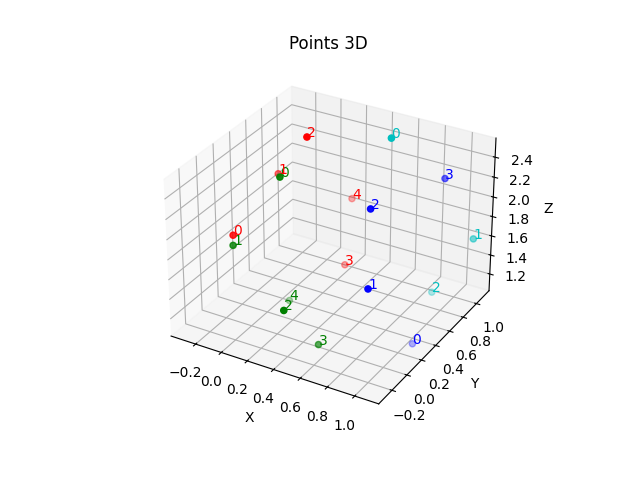
\includegraphics[width=\linewidth]{capture/cloud.png}
    \captionof*{figure}{Nuage de points}
  \end{minipage}
  \hfill
  \begin{minipage}{0.3\linewidth}
    \begin{minipage}{0.4\linewidth}
\fcolorbox{red}{white}{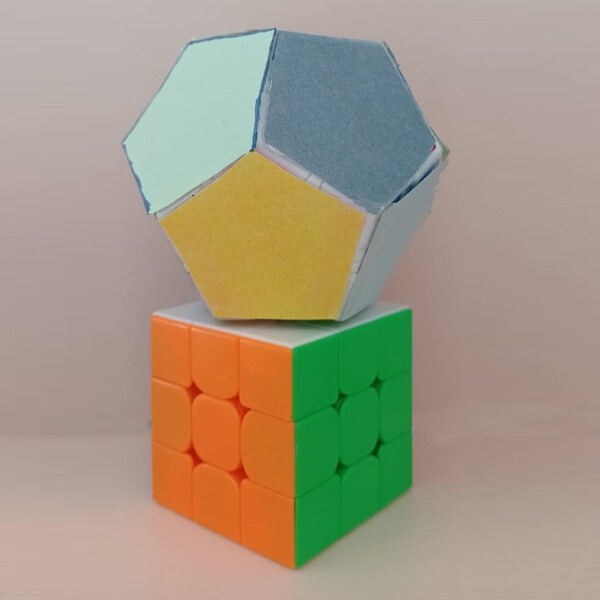
\includegraphics[width=\linewidth]{capture/dodecf1.jpg}}\\[0.5em]
      \fcolorbox{green!50!black}{white}{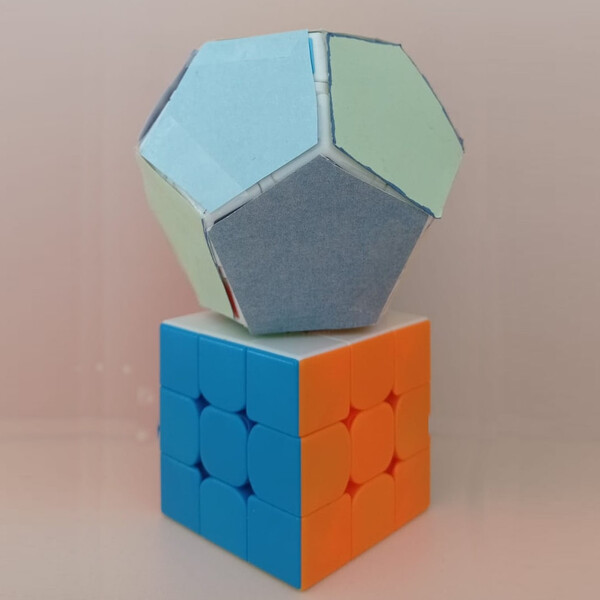
\includegraphics[width=\linewidth]{capture/dodecf3.jpg}}\\[0.5em]
      \fcolorbox{blue!50!black}{white}{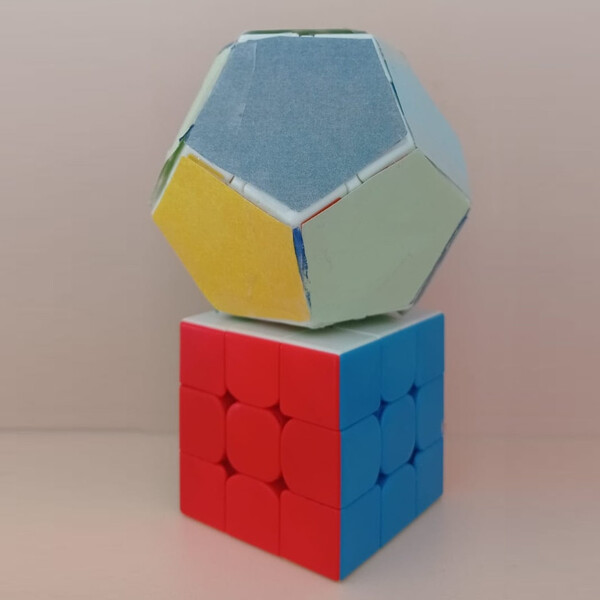
\includegraphics[width=\linewidth]{capture/dodecf5.jpg}}\\[0.5em]
      \fcolorbox{cyan}{white}{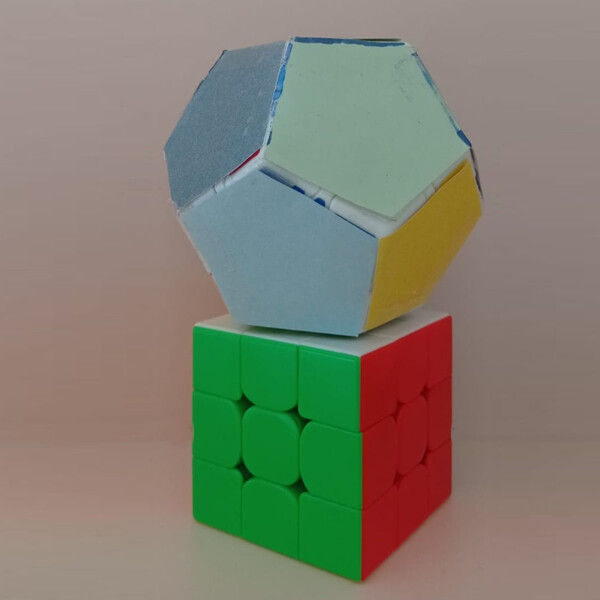
\includegraphics[width=\linewidth]{capture/dodecf7.jpg}}
    \end{minipage}
    \hfill
    \begin{minipage}{0.4\linewidth}
      \fcolorbox{red}{white}{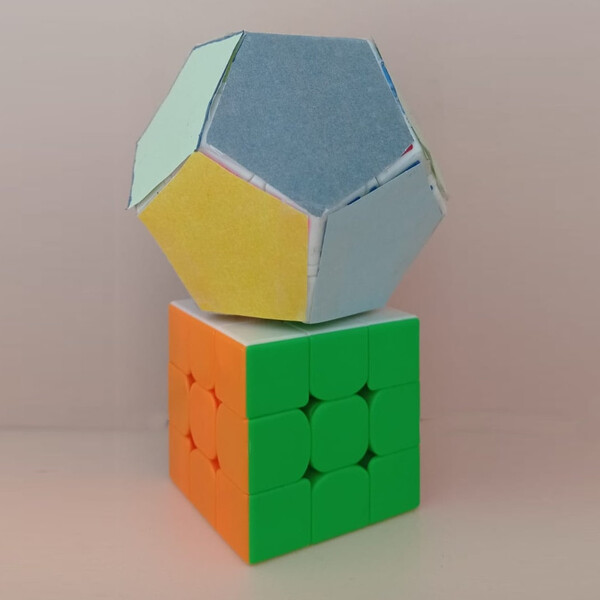
\includegraphics[width=\linewidth]{capture/dodecf0.jpg}}\\[0.5em]
      \fcolorbox{green!50!black}{white}{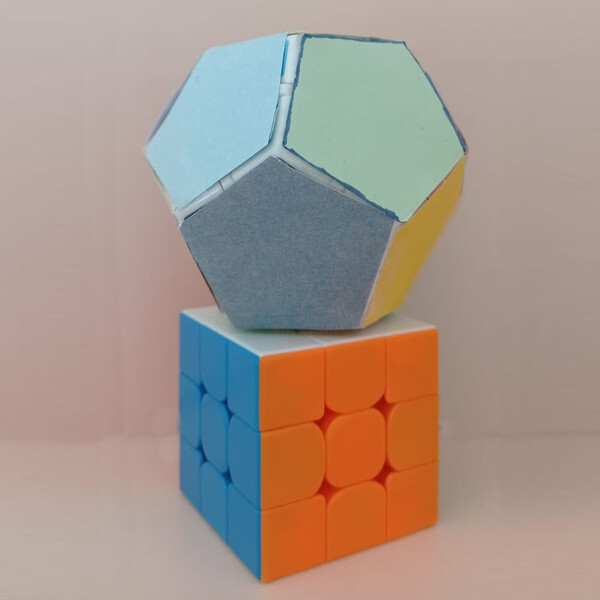
\includegraphics[width=\linewidth]{capture/dodecf2.jpg}}\\[0.5em]
      \fcolorbox{blue!50!black}{white}{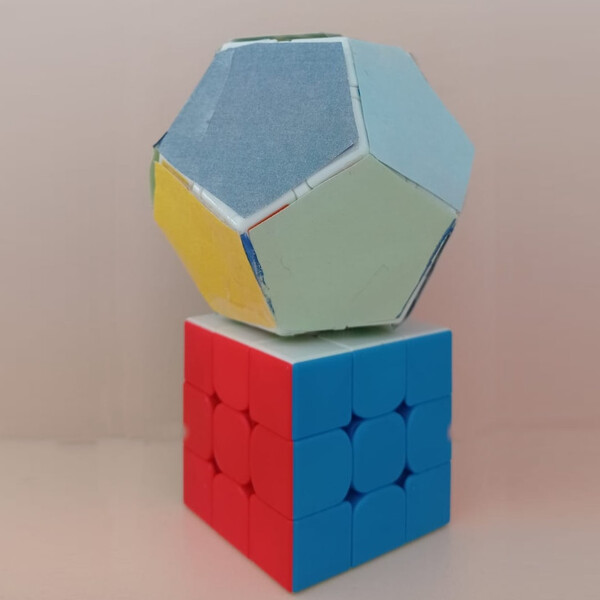
\includegraphics[width=\linewidth]{capture/dodecf4.jpg}}\\[0.5em]
      \fcolorbox{cyan}{white}{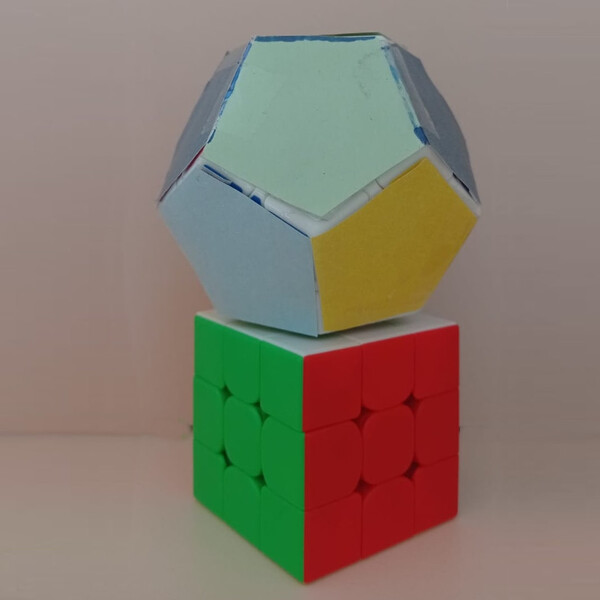
\includegraphics[width=\linewidth]{capture/dodecf6.jpg}}
    \end{minipage}
  \end{minipage}
\end{frame}

\begin{frame}{matrice F}
\end{frame}